\documentclass{standalone}
\usepackage{graphicx}	
\usepackage{amssymb, amsmath}
\usepackage{color}

\usepackage{tikz}
\usetikzlibrary{intersections, backgrounds, math}
\usepackage{pgfmath}

\definecolor{light}{RGB}{220, 188, 188}
\definecolor{mid}{RGB}{185, 124, 124}
\definecolor{dark}{RGB}{143, 39, 39}
\definecolor{highlight}{RGB}{180, 31, 180}
\definecolor{light_teal}{RGB}{107, 142, 142}
\definecolor{mid_teal}{RGB}{72, 117, 117}
\definecolor{dark_teal}{RGB}{29, 79, 79}
\definecolor{gray10}{gray}{0.1}
\definecolor{gray20}{gray}{0.2}
\definecolor{gray30}{gray}{0.3}
\definecolor{gray40}{gray}{0.4}
\definecolor{gray60}{gray}{0.6}
\definecolor{gray70}{gray}{0.7}
\definecolor{gray80}{gray}{0.8}
\definecolor{gray90}{gray}{0.9}
\definecolor{gray95}{gray}{0.95}

\begin{document}

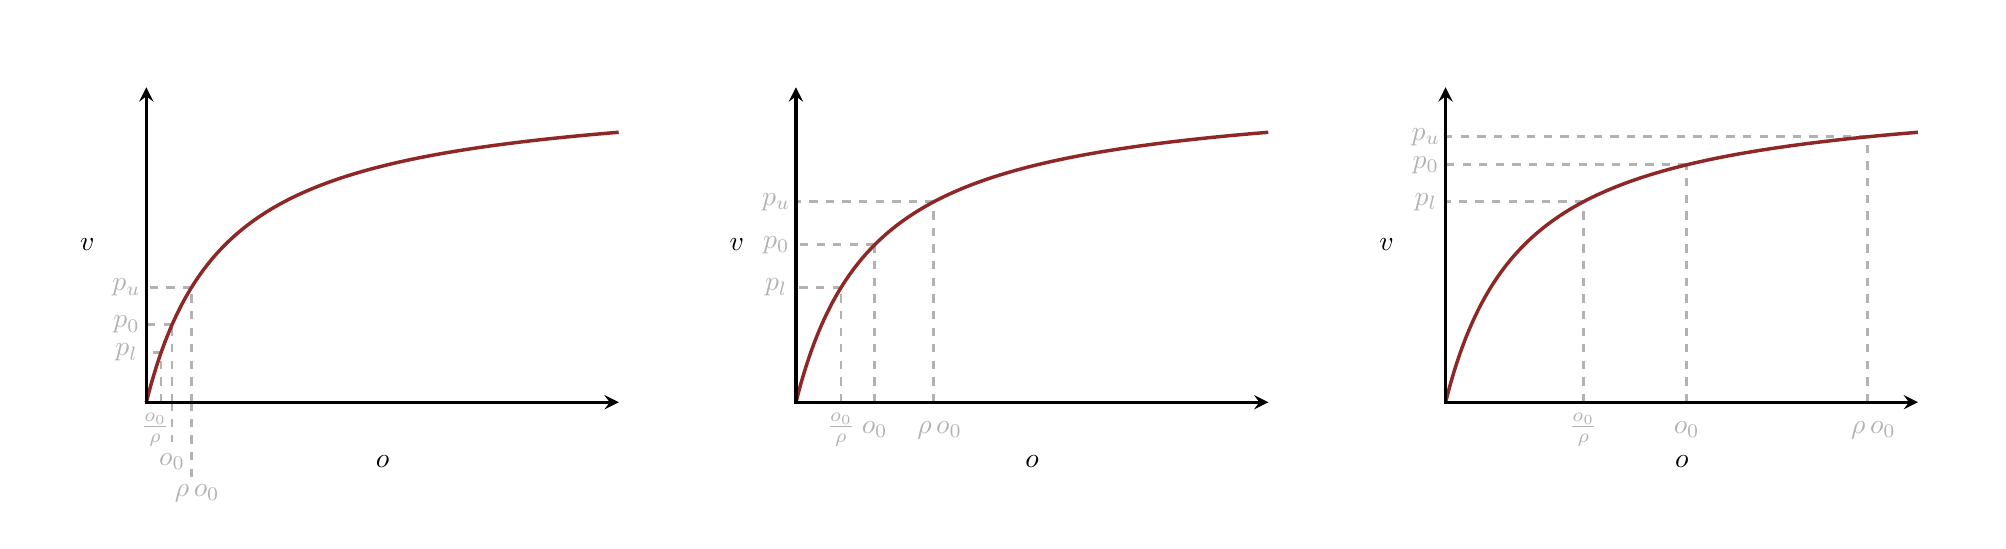
\begin{tikzpicture}[scale=1.0]

  \begin{scope}[shift={(0, 0)}]
    \draw[white] (-1.5, -1.5) rectangle (6.75, 4.75);
        
    \foreach \x in {64/343, 16/49, 4/7} {
      \pgfmathsetmacro{\y}{4 * \x / (1 + \x)}
      \draw[gray70, dashed, line width=1] (\x, 0) -- (\x, \y);
      \draw[gray70, dashed, line width=1] (\x, \y) -- (0, \y);
    }
    
    \pgfmathsetmacro{\x}{64/343}
    \pgfmathsetmacro{\y}{4 * \x / (1 + \x)}
    \draw[gray70, dashed, line width=1] (\x, 0) -- (\x, 0);
    \node[gray70] at (-0.25, \y) { $p_{l}$ };
    \node[gray70] at (\x - 0.075, -0.35) { $\frac{o_{0}}{\rho}$ };
     
    \pgfmathsetmacro{\x}{16/49}
    \pgfmathsetmacro{\y}{4 * \x / (1 + \x)}
    \draw[gray70, dashed, line width=1] (\x, 0) -- (\x, -0.5);
    \node[gray70] at (-0.25, \y) { $p_{0}$ };
    \node[gray70] at (\x, -0.75) { $o_{0}$ };

    \pgfmathsetmacro{\x}{4/7}
    \pgfmathsetmacro{\y}{4 * \x / (1 + \x)}
    \draw[gray70, dashed, line width=1] (\x, 0) -- (\x, -1);
    \node[gray70] at (-0.25, \y) { $p_{u}$ };
    \node[gray70] at (\x + 0.075, -1.15) { $\rho \, o_{0}$ };
    
    \draw[domain={0:6}, smooth, samples=100, line width=1.25, variable=\x, color=dark] 
      plot ({\x},{4 * \x / (1 + \x) });

    \draw [->, >=stealth, line width=1.25] (0, -0.0215) -- (0, 4);
    \draw [->, >=stealth, line width=1.25] (-0.0215, 0) -- (6, 0);
    
    \node at (-0.75, 2) { $v$ };
    \node at (3, -0.75) { $o$ };
  \end{scope}
  
  \begin{scope}[shift={(8.25, 0)}]
    \draw[white] (-1.5, -1.5) rectangle (6.75, 4.75);
        
    \foreach \x in {4/7, 1, 7/4} {
      \pgfmathsetmacro{\y}{4 * \x / (1 + \x)}
      \draw[gray70, dashed, line width=1] (\x, 0) -- (\x, \y);
      \draw[gray70, dashed, line width=1] (\x, \y) -- (0, \y);
    }
    
    \pgfmathsetmacro{\x}{4/7}
    \pgfmathsetmacro{\y}{4 * \x / (1 + \x)}
    \node[gray70] at (-0.25, \y) { $p_{l}$ };
    \node[gray70] at (\x, -0.35) { $\frac{o_{0}}{\rho}$ };
     
    \pgfmathsetmacro{\x}{1}
    \pgfmathsetmacro{\y}{4 * \x / (1 + \x)}
    \node[gray70] at (-0.25, \y) { $p_{0}$ };
    \node[gray70] at (\x, -0.35) { $o_{0}$ };

    \pgfmathsetmacro{\x}{7/4}
    \pgfmathsetmacro{\y}{4 * \x / (1 + \x)}
    \node[gray70] at (-0.25, \y) { $p_{u}$ };
    \node[gray70] at (\x + 0.075, -0.35) { $\rho \, o_{0}$ };
    
    \draw[domain={0:6}, smooth, samples=100, line width=1.25, variable=\x, color=dark] 
      plot ({\x},{4 * \x / (1 + \x) });

    \draw [->, >=stealth, line width=1.25] (0, -0.0215) -- (0, 4);
    \draw [->, >=stealth, line width=1.25] (-0.0215, 0) -- (6, 0);
    
    \node at (-0.75, 2) { $v$ };
    \node at (3, -0.75) { $o$ };
  \end{scope}
  
  \begin{scope}[shift={(16.5, 0)}]
    \draw[white] (-1.5, -1.5) rectangle (6.75, 4.75);
        
    \foreach \x in {7/4, 49/16, 343/64} {
      \pgfmathsetmacro{\y}{4 * \x / (1 + \x)}
      \draw[gray70, dashed, line width=1] (\x, 0) -- (\x, \y);
      \draw[gray70, dashed, line width=1] (\x, \y) -- (0, \y);
    }
    
    \pgfmathsetmacro{\x}{7/4}
    \pgfmathsetmacro{\y}{4 * \x / (1 + \x)}
    \node[gray70] at (-0.25, \y) { $p_{l}$ };
    \node[gray70] at (\x, -0.35) { $\frac{o_{0}}{\rho}$ };
     
    \pgfmathsetmacro{\x}{49/16}
    \pgfmathsetmacro{\y}{4 * \x / (1 + \x)}
    \node[gray70] at (-0.25, \y) { $p_{0}$ };
    \node[gray70] at (\x, -0.35) { $o_{0}$ };

    \pgfmathsetmacro{\x}{343/64}
    \pgfmathsetmacro{\y}{4 * \x / (1 + \x)}
    \node[gray70] at (-0.25, \y) { $p_{u}$ };
    \node[gray70] at (\x + 0.075, -0.35) { $\rho \, o_{0}$ };
    
    \draw[domain={0:6}, smooth, samples=100, line width=1.25, variable=\x, color=dark] 
      plot ({\x},{4 * \x / (1 + \x) });

    \draw [->, >=stealth, line width=1.25] (0, -0.0215) -- (0, 4);
    \draw [->, >=stealth, line width=1.25] (-0.0215, 0) -- (6, 0);
    
    \node at (-0.75, 2) { $v$ };
    \node at (3, -0.75) { $o$ };
  \end{scope}
    
\end{tikzpicture}

\end{document}  